% Kapitel ch:mr: Lead, Setup, Results & Discussion. Setting steht in docs/introduction_v2.tex,
% Discussion in docs/discussion_omol25.md (Conclusion & Outlook).
% Einzige Quelle fuer den Kapiteltext; section_results.tex und
% section_results_merged.tex sind abgeloest.
%
% Gruppennamen: closed-shell (<S^2> = 0) und broken-symmetry (<S^2> > 0),
% klassifiziert nach der Einzelpunktrechnung mit Stabilitaetsanalyse.
% "RKS instability" nur dort, wo der Stabilitaetstest beschrieben ist.
% "restricted surface" / "unrestricted surface" sind Flaechen, keine Gruppen.
%
% Figuren: Pictures/Fig1_v2.png, Pictures/fig2_force_mae.png, Pictures/fig3_v2.png
% aus pipeline/plot_paper_figs_v2.py. Zahlen aus results/*.csv, geprueft mit
% pipeline/check_results_section.py.

\chapter{Higher-Fidelity Relabelling Without Re-optimising the Path Is Not Enough}
\label{ch:mr}

\emph{The opening of this chapter, up to Section~\ref{sec:omol-setup},
briefly recaps the introduction and links Chapter~\ref{ch:delta} to
this one.}

The introduction asked two questions: whether a model can be lifted
to a higher level of theory by relabelling only a subset of its
training data (RQ1), and whether a model can learn a surface from
paths that were never relaxed on that surface (RQ2).
Chapter~\ref{ch:delta} answered RQ1. For that chapter, RQ2 needed no
test: both levels of theory are restricted, and the transition states
optimised at the two levels differ by a median RMSD of only
0.007\,\AA{}. Paths relaxed at the lower level therefore already sample
the transition-state region of the higher one, and relabelling the
paths without re-optimising them is enough.

This stops being true when the spin formalism changes as well. At a
broken-symmetry transition state the restricted solution is unstable
(Section~\ref{sec:background-stability}), and the transition
state found unrestricted can lie far from the one found restricted in
configuration space. A path relaxed restricted then may no longer
sample the transition-state region of the unrestricted surface, and RQ2
becomes a real question.

A subset-relabelling approach like that of Chapter~\ref{ch:delta}
cannot answer it: a failure of
the corrected model could come from the head and its small training
set, or from the training paths holding no transition state of that
surface, and the two cannot be told apart. We therefore leave the
correction head and the subset training behind and turn to OMol25, a
dataset of more than 100 million DFT calculations. It takes over the
geometries of many existing datasets, generated at lower levels of
theory, and recomputes only their labels. Transition1x is one of them:
it was relabelled in full (training, validation and test split alike,
all in the OMol25 training split), with every label recomputed
unrestricted at a higher level. We train nothing ourselves: we take three published
models trained on OMol25, UMA-S, UMA-M and eSEN, and test them. Every
label is relabelled and the models are large ones trained on all of it,
so neither a subset nor a small head can be blamed for a failure. What
remains is the training paths, which were never relaxed on the surface
of their labels; that is RQ2 (Table~\ref{tab:delta-vs-omol}).

\begin{table}[H]
\centering
\small
\caption{The two relabelling setups of this thesis. The Transition1x
paths are in both, unchanged; everything else is stronger in the
second.}
\label{tab:delta-vs-omol}
\resizebox{\linewidth}{!}{%
\begin{tabular}{@{}llp{5.5cm}@{}}
\toprule
 & Chapter~\ref{ch:delta} & this chapter \\
\midrule
training data & Transition1x & OMol25: Transition1x and about 100 million further structures \\
paths re-optimised at the new level & no & no \\
labels recomputed & under 1\,\% of Transition1x & all \\
spin formalism of the labels & restricted & unrestricted \\
level of the labels & $\omega$B97M-V/def2-TZVP & $\omega$B97M-V/def2-TZVPD \\
model & MACE with a correction head & UMA-S, UMA-M, eSEN \\
\bottomrule
\end{tabular}}
\end{table}

Whether these models find broken-symmetry transition states has not
been tested systematically: the published benchmarks report high
success rates for them~\cite{marks2026, hait2025}, but they score the
models against restricted references, and the few broken-symmetry cases
they met were removed or left unchecked
(Chapter~\ref{ch:introduction}, Appendix~\ref{app:marks}). This chapter
runs that test.

From the Transition1x test split, which is held out for MACE but part
of the OMol25 training data, we select reactions where
broken-symmetry transition states are expected, let the three models
search them, and re-evaluate every transition state found with
unrestricted DFT and a stability analysis, which sorts the structures
into closed-shell and broken-symmetry. The models' predictions are
measured against the DFT forces and energies of this re-evaluation, and
we then compare whether the models perform differently at the
broken-symmetry transition states than at the closed-shell ones.

\section{Setup}
\label{sec:omol-setup}

\subsection{Reactions selected stratified by multireference character}
\label{sec:reactions}
The reactions are selected as in Chapter~\ref{ch:delta}, from the
same ranking (Section~\ref{sec:delta-protocol}), only with a larger
high-MR group; the selection is described in full here so that this
chapter can be read on its own. The Transition1x test split contains
287 reactions. A broken-symmetry
transition state is expected where the multireference character is
high, so we rank the reactions by it and select from both ends and the
middle: a large high-MR group, where broken-symmetry transition states
should be frequent; a low-MR group, where the restricted solution
should be stable throughout, as control; and a mid-MR group
in between.

We quantify MR character by $N_\mathrm{FOD}$, evaluated at a geometry in the
transition-state region, where we expect the multireference character to be
highest. To obtain such a geometry we use a restricted
\mbox{$\omega$B97M-V/def2-TZVP} NEB. It converges for 279 of the 287
reactions; the remaining eight are discarded from the ranking and
from every step that follows.

We compute $N_\mathrm{FOD}$ at these transition states (PBE/def2-SVP, Fermi
smearing, $T_\mathrm{el} = 5000$~K; see
Section~\ref{sec:background-beyond} for details), rank the reactions by
it, and select 26 high-MR reactions from the top of the ranking, 9 mid-MR
reactions spread across the middle, and 10 low-MR reactions from the
bottom\footnote{The high stratum takes ranks 1--26, the low stratum ranks
270--279, and the mid stratum is drawn at ten evenly spaced ranks
($11, 40, 68, \dots, 269$). Rank 11 already lies inside the top 26, so the mid
stratum contributes nine distinct reactions and the union is 45 rather than 46.
The high stratum is the largest because it is the regime under test; the other
two serve as reference points at the opposite end and across the interior.}
(Table~\ref{tab:strata}).

The 45 reactions are unimolecular CHNO reactions of 10 to 14 atoms, all neutral
singlets, spanning five stoichiometries and mostly belonging to two isomer
families, C$_3$H$_5$NO$_2$ (22 reactions) and C$_5$H$_5$NO (16).


\begin{table}[H]
\caption{The benchmark set, curated from the $N_\mathrm{FOD}$ ranking of
the 279 converged test-split reactions. One reaction falls in both the
high- and mid-MR group, giving 45 reactions in total.}
\label{tab:strata}
\centering
\begin{tabular}{lrrl}
\toprule
Group & $n$ & Ranks & $N_\mathrm{FOD}$ \\
\midrule
high MR & 26 & 1--26            & 0.68--1.15 \\
mid MR  &  9 & 40--269, uniform & 0.02--0.57 \\
low MR  & 10 & 270--279         & 0.003--0.014 \\
\bottomrule
\end{tabular}
\end{table}

$N_\mathrm{FOD}$ serves one purpose here: it selects the reactions
where a broken-symmetry transition state is likely. It is an estimate,
computed at one geometry per reaction before any model has run, and
it does not say whether the broken-symmetry solution is actually
there. Once the models have delivered their transition states, that
can be measured directly, at the geometry being tested: the
$\langle S^2\rangle$ of the DFT single point (Section~\ref{sec:dft})
says whether the lowest solution there is closed-shell or
broken-symmetry. From here on we therefore classify by
$\langle S^2\rangle$, and the $N_\mathrm{FOD}$ groups appear again
only to check that the selection worked
(Section~\ref{sec:classification}).


\subsection{Transition-State Searches with OMol25 MLIPs}
\label{sec:neb}

We use three OMol25 models, the MLIPs trained on OMol25 by Meta FAIR
(Section~\ref{sec:model-uma-esen}): UMA-S (\texttt{uma-s-1p2}), UMA-M
(\texttt{uma-m-1p1}) and eSEN (\texttt{esen-sm-conserving-all}). Each
is used to search the transition state and evaluate the barrier height by running one CI-NEB per model on each of the
45 reactions, for 135 searches in total (fairchem 2.20.0, ASE 3.28.0). All three
run on the \texttt{omol} task head at charge 0 and spin multiplicity 1. %matching the neutral singlet the DFT side treats.

\textbf{Band initialisation:} We initialise each band with the final \mbox{$\omega$B97X/6-31G(d)} band stored in
Transition1x, ten images including reactant and product, and re-relax the two
endpoints with the respective model (BFGS, $0.05$~eV\,\AA$^{-1}$).

\textbf{Settings for NEB run:} Optimisation used the improved-tangent method, ASE's default spring constant of
$0.1$~eV\,\AA$^{-2}$ on each of the nine springs, and the adaptive ordinary
differential equation (ODE) solver of ASE's \texttt{NEBOptimizer}
(\texttt{ode12r}~\cite{makri2019preconditioning}). We ran first without a
climbing image to a maximum NEB force of $f_\mathrm{max} = 0.15$~eV\,\AA$^{-1}$ on the band,
then with the climbing image to $0.05$~eV\,\AA$^{-1}$, at most 500 optimiser
steps per phase.


% S. Makri, C. Ortner and J. R. Kermode, J. Chem. Phys. 150, 094109 (2019) https://dx.doi.org/10.1063/1.5064465

Of the 135 bands, 112 reached $f_\mathrm{max} < 0.05$~eV\,\AA$^{-1}$;
the other 23 did not. The optimiser nevertheless reported success in
133 of the 135 searches, because running out of steps raises no
error. We report all 135, because what we measure is the transition
state an MLIP actually delivers, and leaving the 23 out does not
change the force results: the ratio between the two groups moves from
$2.55$ to $2.45$; for the barrier spread see
Section~\ref{sec:results-barrier}.\footnote{The 112 converged after a
median of 66 optimiser steps. The other 23 stopped between $0.070$
and $0.319$~eV\,\AA$^{-1}$: 21 at the step limit, after a median of
478 steps, and two aborted by the solver. Restricting every analysis
to the 112 leaves the median DFT residual force at the transition state
unchanged for closed-shell structures ($0.051$~eV\,\AA$^{-1}$) and lowers it
slightly for broken-symmetry ones ($0.129$ to $0.124$), so the ratio between the
two groups moves from $2.55$ to $2.45$.}


\subsection{The DFT Reevaluation on the Model Transition State}
\label{sec:dft}

At the end of a search the workflow reports a transition state found
by the model. We check that structure with one unrestricted DFT
single point at the geometry the model found, without re-optimising
it. The single point gives three things:

\begin{itemize}
  \item the DFT forces. They show whether the structure is a stationary
    point of the surface the labels describe: at a stationary point the
    force is zero, and a large force means the model stopped somewhere
    else. The deviation of the model forces from the DFT forces is the
    force error.
  \item the DFT energy. It gives the barrier of the model's own
    geometries on that surface. The deviation of the model barrier from
    the DFT barrier is the energy error.
  \item $\langle S^2\rangle$: whether that surface is closed-shell or
    broken-symmetry at this geometry. This is the classification of
    Section~\ref{sec:classification}.
\end{itemize}

No DFT transition-state search enters this comparison.

\paragraph{Protocol.} The single point uses the electronic structure
settings under which the OMol25 labels were generated:
\mbox{$\omega$B97M-V/def2-TZVPD}, unrestricted, with def2/J, RIJCOSX,
TightSCF and DEFGRID3 (Table~\ref{tab:protocol}).\footnote{ORCA input:
\texttt{! UKS wB97M-V def2-TZVPD def2/J RIJCOSX TightSCF DEFGRID3},
\texttt{\%scf Thresh 1e-12 TCut 1e-13 MaxIter 300 end}, charge 0,
multiplicity 1. The forces are taken from a separate \texttt{EnGrad}
calculation that reads the converged orbitals of the single point
through \texttt{MORead}; re-converging from a default guess could land
on the restricted solution instead, which would place the gradient on a
different surface than the classification.} The models learned this
surface, so the check has to run on it. One thing is changed
deliberately: the route to the broken-symmetry solution. OMol25
rotates the HOMO and LUMO of the starting guess by $20^\circ$ in the
$\beta$ space, hoping to land on a broken-symmetry solution if one
exists. A closed-shell result could then also mean that the SCF fell
back to the restricted solution after the rotation. We instead let
the SCF converge unperturbed, which for a singlet gives the
restricted solution (Section~\ref{sec:background-stability}).
\texttt{STABPerform} then tests whether a lower broken-symmetry
solution exists, and where it does, \texttt{STABRestartUHFifUnstable}
restarts from orbitals displaced along the unstable direction and
converges onto it. A closed-shell
result now means that no lower solution exists. OMol25's route can
miss a broken-symmetry solution, ours cannot.

\paragraph{Terminology.} \emph{Energies and forces of the solution the
run settles on are those of the unrestricted surface of
Section~\ref{sec:background-stability}: the lowest unrestricted
solution, checked by stability analysis, which for a closed-shell
structure coincides with the restricted surface. The chapter uses
``unrestricted surface'' in this sense throughout.}

\begin{table}[H]
\caption{Electronic structure protocol of the OMol25 labels and of the labels
in this work. Two rows differ: how the broken-symmetry solution is reached,
which we changed deliberately, and the ORCA version. Both differences were
tested.}
\label{tab:protocol}
\centering
\small
\begin{tabular}{@{}l >{\raggedright\arraybackslash}p{4.8cm}
                     >{\raggedright\arraybackslash}p{4.4cm}@{}}
\toprule
 & OMol25 labels & Labels in this work \\
\midrule
Functional / basis         & $\omega$B97M-V / def2-TZVPD & same \\
Auxiliary basis, integrals & def2/J, RIJCOSX             & same \\
Grid, thresholds           & DEFGRID3, Thresh $10^{-12}$, TCut $10^{-13}$ & same \\
SCF settings               & unrestricted, TightSCF      & same \\
Charge, multiplicity       & 0, 1                        & same \\
\midrule
Symmetry breaking          & before the SCF: HOMO and LUMO of the guess
                             rotated by $20^\circ$
                             \newline \emph{tries to find a broken-symmetry
                             solution}
                           & after the SCF: converged solution tested for
                             stability, restarted if unstable
                             \newline \emph{checks whether one exists} \\
Consequence                & can miss a lower solution that exists;
                             a closed-shell result is ambiguous
                           & a closed-shell result means no lower
                             solution exists \\
ORCA version               & 6.0.0                       & 5.0.4 \\
\bottomrule
\end{tabular}
\end{table}

\paragraph{Validation of the protocol.} Our protocol differs from
OMol25's in two points, the route to the broken-symmetry solution and
the ORCA version (Table~\ref{tab:protocol}). Both were tested.
The route to the broken-symmetry solution was tested on the 135 model
transition states. There we ran
the OMol25 rotation next to our stability analysis. The two agree on
134 structures, to within $4.1\cdot10^{-7}$~Ha in total energy. In the
one exception the rotation stayed closed-shell and the stability
analysis found a solution $7.1$~meV lower; no structure shows the
reverse. The two routes thus reach the same solution, and where they
differ ours finds the lower one. The version difference was tested against the published OMol25
labels of our Transition1x transition states.\footnote{Published
labels exist only for the geometries OMol25 took over; 44 of our 45
transition states are in the release.} Our 5.0.4 single points and
the published 6.0.0 labels agree to under $0.1$~meV in energy and
$0.02$~eV\,\AA$^{-1}$ in force, and at all 17 broken-symmetry
geometries the OMol25 label sits on the broken solution.


\subsection{Classification: closed-shell or broken-symmetry}
\label{sec:classification}

As described above, the DFT single point also provides the
$\langle S^2\rangle$ of the solution the run settles on. We use that
measurement to group the transition states the models deliver into
closed-shell and broken-symmetry. A structure with $\langle S^2\rangle = 0$ is
closed-shell, one with $\langle S^2\rangle > 0$ is broken-symmetry. That
gives 82 closed-shell and 53 broken-symmetry structures, with no
borderline case: the smallest non-zero value is $0.0579$. This
grouping is used in every result of the chapter.

One quantity, the spread of the DFT barrier over the three model
geometries of a reaction (Fig.~\ref{fig:barrier}B), is defined per
reaction rather than per structure and needs a class per reaction: a
reaction counts as broken-symmetry if at least one of its three
transition states is, which gives 18 broken-symmetry and 27
closed-shell reactions.

The classification also checks the selection of
Section~\ref{sec:reactions}, which ranked the reactions by
$N_\mathrm{FOD}$. It did what it was supposed to: 17 of the 26 high-MR reactions are broken-symmetry, 1 of
the 9 mid-MR reactions, and none of the 10 low-MR
ones.\footnote{The same check serves Chapter~\ref{ch:delta}, whose
overshoot at high MR was left unexplained there. The 30 reactions of
Chapter~\ref{ch:delta} are all among the 45; at their Transition1x
transition states (Section~\ref{sec:labels}) the lowest solution is
broken-symmetry for seven of the ten high-MR, one of the ten mid-MR
and none of the ten low-MR reactions of that chapter.}

\paragraph{Breaking depth.} Whether a broken-symmetry solution exists
is a yes-or-no answer. How far it lies below the restricted solution,
the breaking depth $E_\mathrm{RKS} - E_\mathrm{BS}$
(Section~\ref{sec:background-stability}), is a second number. We
need it later to test whether the models' errors grow with the depth
or only with the existence of a lower broken-symmetry solution
(Section~\ref{sec:results-ferr}). The depth needs two energies at the
same geometry. $E_\mathrm{BS}$ is already there: it is the energy of
the unrestricted run of Section~\ref{sec:dft}. $E_\mathrm{RKS}$ takes
one more calculation, a restricted single point at the same geometry
and level, run without a stability analysis so that it stays on the
restricted solution. We ran it for the 53 broken-symmetry structures. For
the closed-shell structures the depth is zero by construction, since
the stability analysis has found no lower
solution.\footnote{One closed-shell structure was run anyway as a
control: it comes out at $0.0008$~meV.}

\subsection{Residual forces at the training geometries}
\label{sec:labels}

The previous subsections describe how the transition states delivered
by the models are examined. This one turns to the data the models were
trained on. If the models fail at broken-symmetry transition states, a
suspected cause is the training data, whose paths were never relaxed on
the surface their labels describe. Here we measure how far they are
from stationarity on that surface. We do so at the stored transition
states of our 45 reactions: the transition-state geometry that
Transition1x holds for each reaction, relaxed restricted at
\mbox{$\omega$B97X/6-31G(d)}. OMol25 took these geometries over
unchanged and relabelled them, so they are part of the models' training
data.

\paragraph{Terminology.} \emph{From here on, the Transition1x level is
\mbox{$\omega$B97X/6-31G(d)} and the OMol25 level
\mbox{$\omega$B97M-V/def2-TZVPD}. A level names
functional and basis only; the spin formalism is stated separately, as
the restricted or the unrestricted surface. A surface is fixed by both,
the level and the spin formalism, and changing either one gives a
different surface.}

Ideally, the geometries in a training set for transition-state search
are relaxed on the surface their labels describe. Transition1x
satisfies this: paths and labels share the restricted surface at the
Transition1x level. OMol25 kept the geometries and recomputed the labels
on the unrestricted surface at the OMol25 level
(Table~\ref{tab:t1x-vs-omol-labels}), so neither the level of theory nor
the spin formalism of a label matches that of its geometry. Stationary
points are specific to a surface: the stored transition states are not
necessarily stationary points of the label surface, whose transition
state may lie elsewhere in configuration space. A model learns the surface its
labels describe, so it has to learn the label surface from points
displaced from its transition state rather than from the transition
state itself.
Figure~\ref{fig:pes} sketches this for a broken-symmetry
reaction.\footnote{The label ``all iterations'' in the figure is a
simplification: Transition1x kept a band only when it differed enough
from the last one kept (Section~\ref{sec:dataset-t1x}).}

\begin{table}[H]
\centering
\small
\caption{Where the Transition1x transition-state geometries were
relaxed, and where their labels were computed, in the two datasets.}
\label{tab:t1x-vs-omol-labels}
\begin{tabular}{@{}lllll@{}}
\toprule
 & \multicolumn{2}{c}{geometry relaxed} & \multicolumn{2}{c}{label computed} \\
\cmidrule(lr){2-3} \cmidrule(l){4-5}
 & level of theory & spin formalism & level of theory & spin formalism \\
\midrule
Transition1x & $\omega$B97X/6-31G(d) & restricted & $\omega$B97X/6-31G(d) & restricted \\
OMol25       & $\omega$B97X/6-31G(d) & restricted & $\omega$B97M-V/def2-TZVPD & unrestricted \\
\bottomrule
\end{tabular}
\end{table}

To quantify how far the stored transition states are from stationarity
on the label surface, we use the residual force: the largest force
component on the atoms at the stored geometry, evaluated on the label
surface. It vanishes at a stationary point of the surface. A non-zero
value shows that the stored geometry is not a stationary point, and its
magnitude measures how far from stationarity the geometry is.

We measure the residual force at the 45 Transition1x transition
states in three steps (Figure~\ref{fig:ladder-protocol}): at the Transition1x level, as stored with the
dataset; at the OMol25 level on the restricted surface; and at the
OMol25 level on the unrestricted surface (Sec.~\ref{sec:dft}). The first step confirms that the
geometries are relaxed at their own level. The second isolates what
the change of level from \mbox{$\omega$B97X/6-31G(d)} to
\mbox{$\omega$B97M-V/def2-TZVPD} does, the third what the change of spin
formalism from restricted to unrestricted does.
As a control, we re-optimise the transition states at the OMol25
level on the restricted surface\footnote{CI-NEB with the band protocol of the
model searches. Of the 45 bands, 33 reached the force criterion; the twelve
that did not (nine closed-shell, three broken-symmetry) stopped between
$0.059$ and $0.117$~eV\,\AA$^{-1}$.} and repeat steps 2 and 3 at the
re-optimised geometries. If the spin-formalism effect survives, it is
not a leftover of the level change.

\begin{figure}[H]
  \centering
  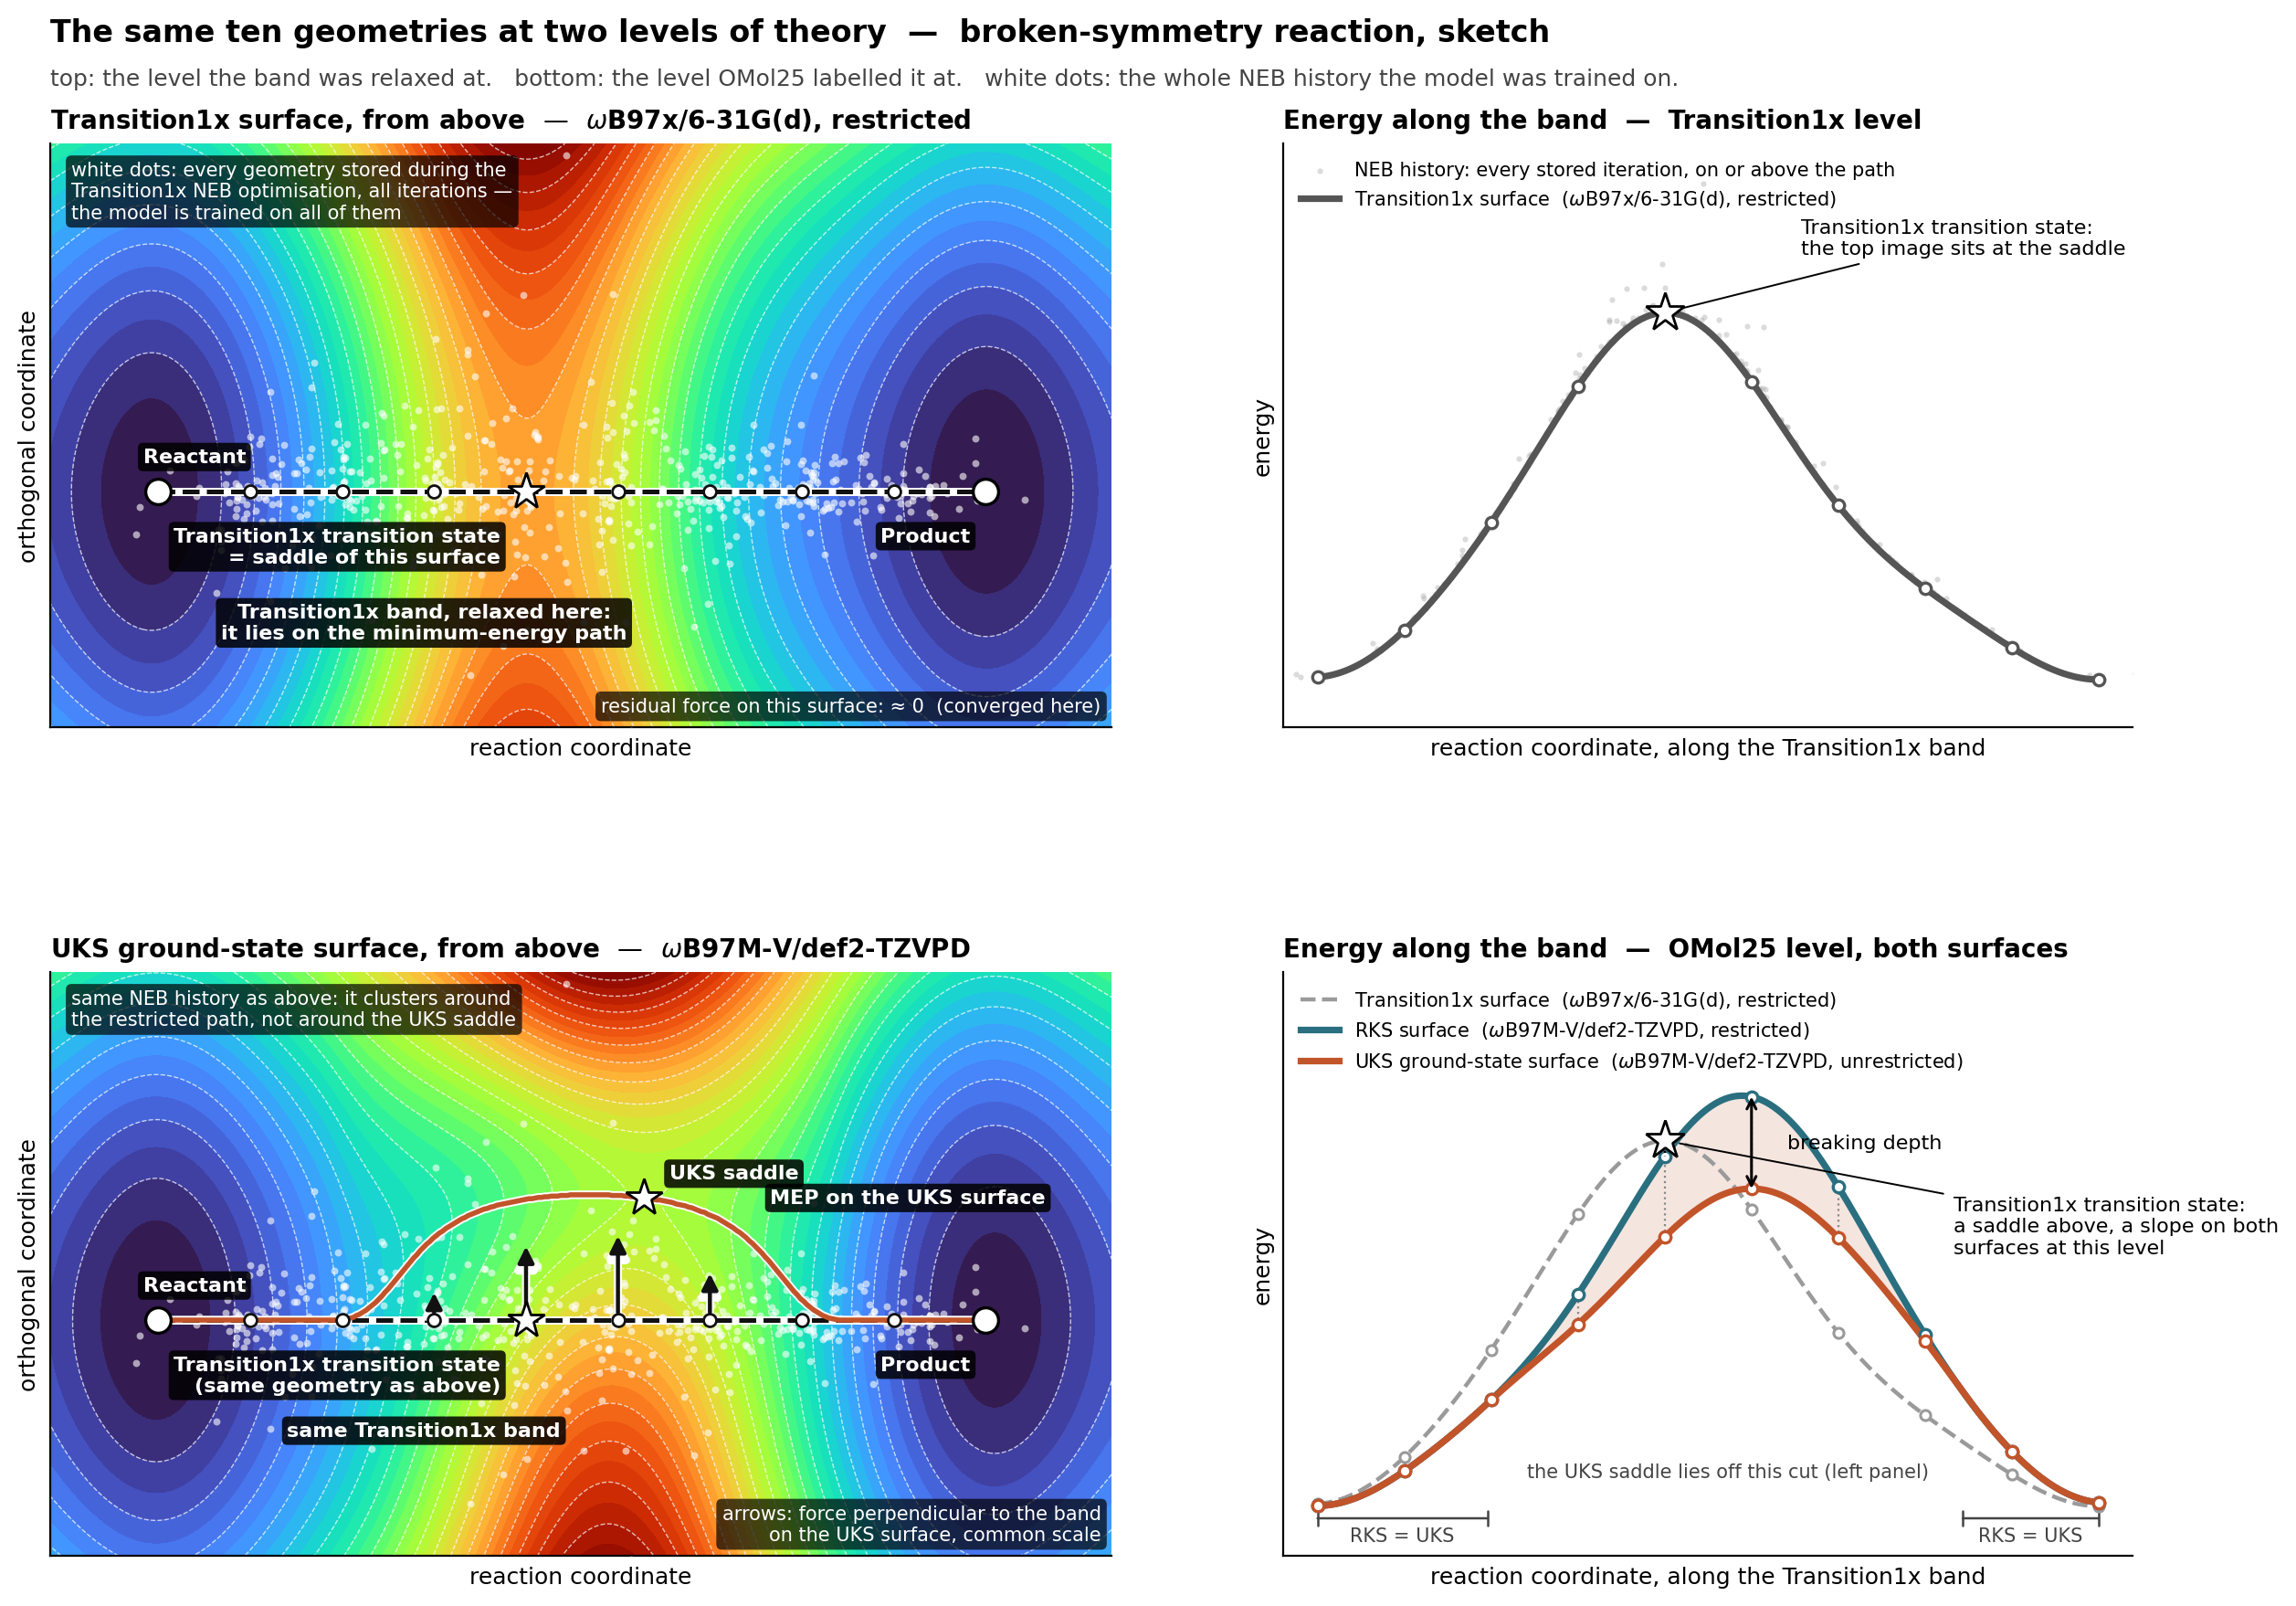
\includegraphics[width=\textwidth]{Pictures/fig_pes.png}
  \caption{Schematic of the mechanism, not a computed surface. The same
  geometries of a broken-symmetry reaction are shown on the restricted
  surface they were relaxed on (top) and on the unrestricted surface
  the labels were computed on (bottom). On the restricted surface the
  transition state is a saddle and the band with its stored NEB history
  (white dots) lies on the minimum-energy path. On the unrestricted
  surface the same band lies on a slope, the force at the transition
  state is not zero (arrows), and the saddle lies elsewhere. Right: the
  energy along the band on each surface.}
  \label{fig:pes}
\end{figure}

\begin{figure}[H]
  \centering
  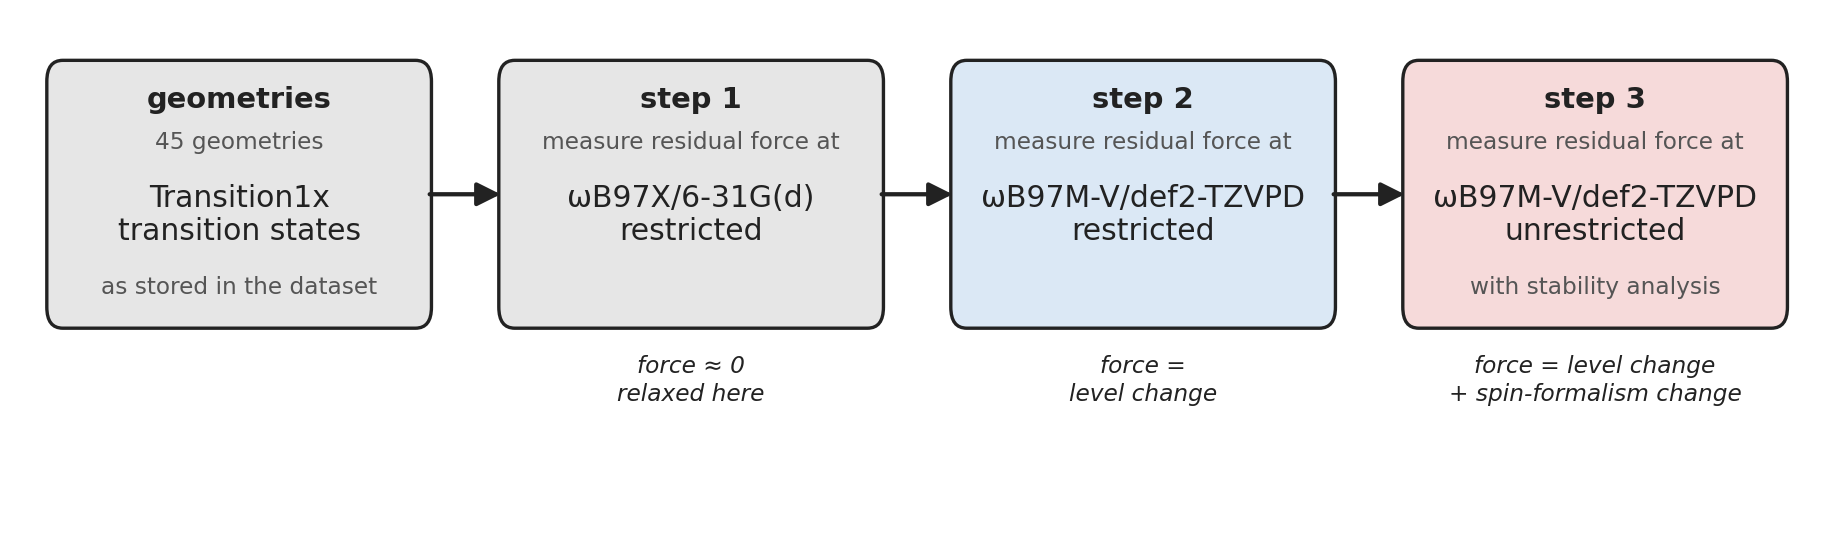
\includegraphics[width=\textwidth]{Pictures/fig_ladder_protocol_v5.png}
  \caption{The residual-force protocol of Section~\ref{sec:labels}: the
  stored Transition1x transition states are evaluated three times,
  adding one change at a time. The columns are those of
  Table~\ref{tab:ladder}.}
  \label{fig:ladder-protocol}
\end{figure}

\section{Results \& Discussion}
\subsection{The model underestimates the residual force at broken-symmetry transition states}
\label{sec:results-silent}

Figure~\ref{fig:silent} shows, for all 135 model transition states, the
residual force according to the model against the residual force from the DFT
re-evaluation at the identical geometry (Sec.~\ref{sec:dft}). The
residual force is the largest force component at that geometry,
$\max_i |F_i|$ over all $3N$ Cartesian components, the same
$f_\mathrm{max}$ the NEB converges on
(Section~\ref{sec:background-neb}). Colours mark
the two groups of Section~\ref{sec:classification}: 82 closed-shell and 53
broken-symmetry structures.

\begin{figure}[H]
  \centering
  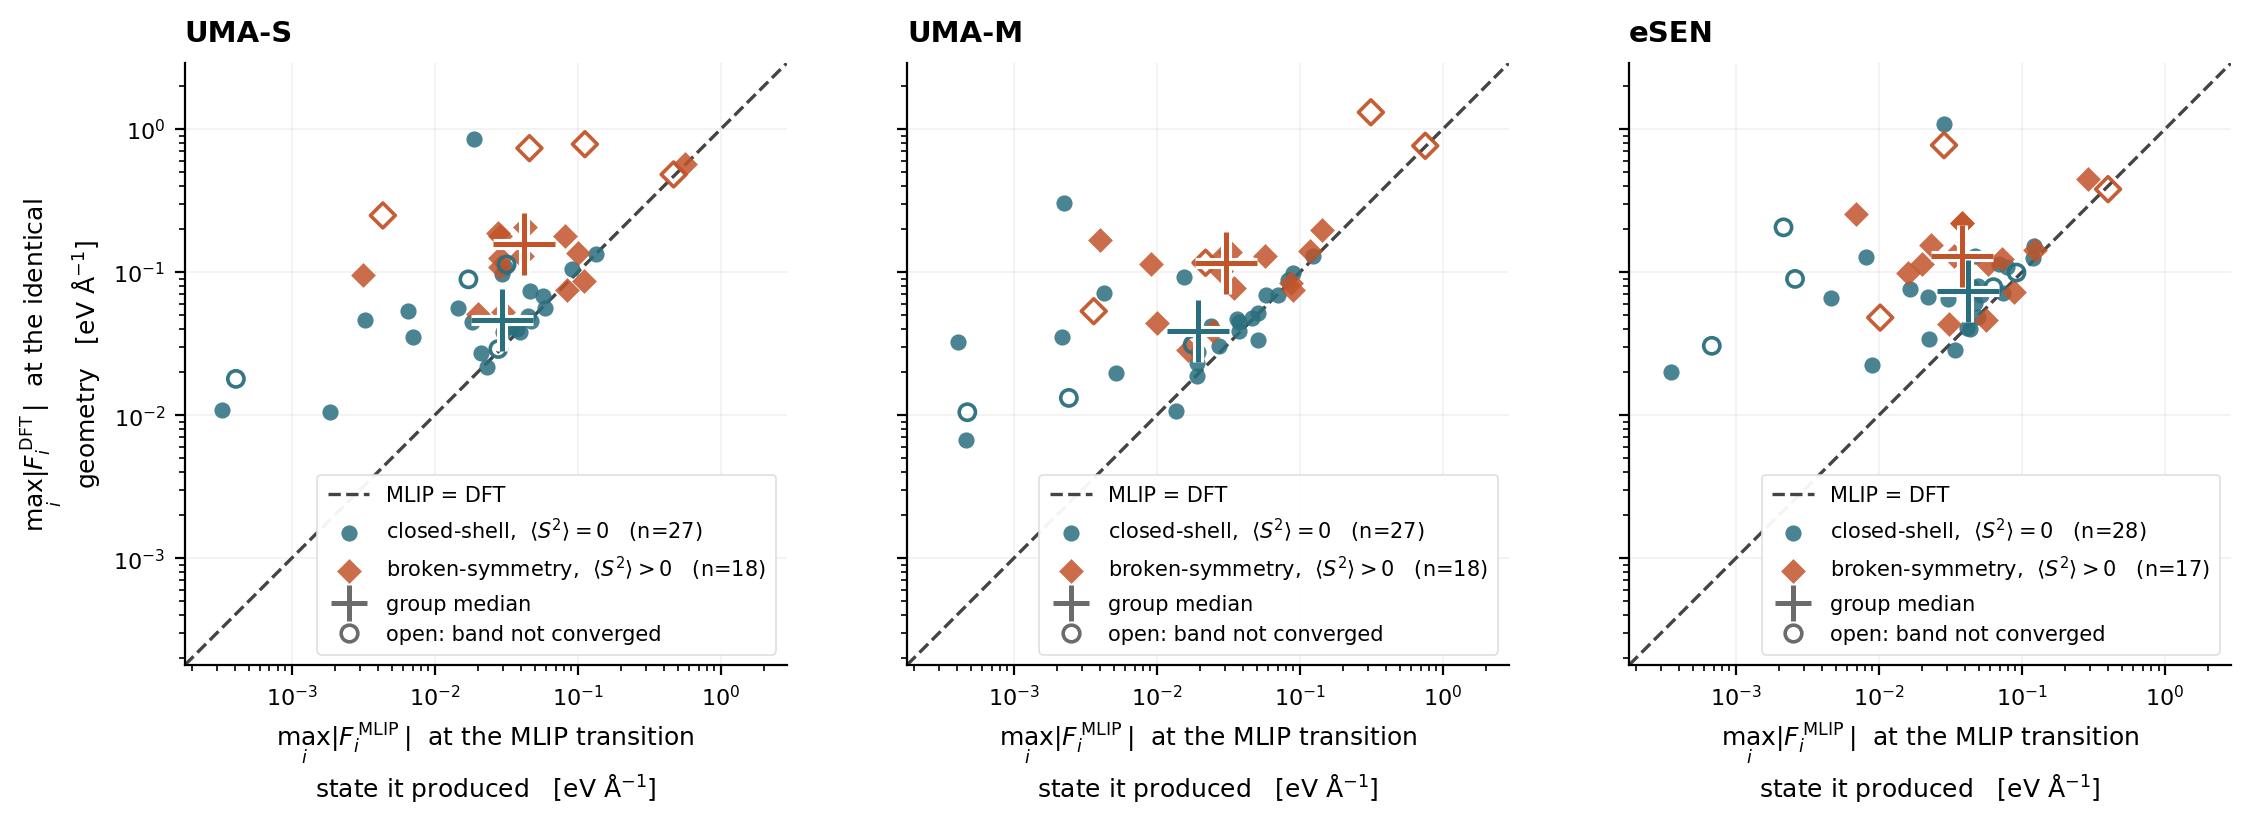
\includegraphics[width=\linewidth]{Pictures/Fig1_v2.png}
  \caption{Residual force at the transition state each model delivered,
  according to the model against DFT at the same unrelaxed geometry
  (45~reactions $\times$ 3~models, all 135 structures). Both axes give
  the largest force component, $\max_i |F_i|$. DFT at the OMol25 level
  on the unrestricted surface (Sec.~\ref{sec:dft}). Colours mark the two
  groups of Section~\ref{sec:classification}, 82 closed-shell and 53
  broken-symmetry structures; crosses are the group medians per model.
  Open markers: the band of that search did not reach the convergence
  criterion (Sec.~\ref{sec:neb}); the medians include them.}
  \label{fig:silent}
\end{figure}

According to the model, both groups are equally converged: the median
residual force is 0.0299~eV\,\AA$^{-1}$ at the closed-shell structures and
0.0344 at the broken-symmetry ones, a factor of 1.15. For eSEN the
broken-symmetry structures even come out slightly lower (0.038 against 0.042).

But when checked with DFT, they are not. The median residual force is
0.0507~eV\,\AA$^{-1}$ at the closed-shell structures and 0.1293 at the
broken-symmetry ones --- 2.55 times larger. Every model shows the same gap:
UMA-S 0.046 against 0.157, UMA-M 0.039 against 0.115, eSEN 0.074 against
0.129.\footnote{Restricting to the 112 searches that met the band
criterion gives 2.45 for the DFT separation and 1.03 for the model
separation.}

The failure is silent. The model's own residual force is the only
convergence signal in the workflow, and it is the same for both
groups, so nothing in a search tells a broken-symmetry structure that
is off the saddle from a closed-shell one that is on it. Only the DFT
check shows the difference.


\subsection{The force error is larger at broken-symmetry transition states, by a factor of two to three}
\label{sec:results-ferr}

Figure~\ref{fig:silent} and the subsection above asked whether the
model's transition state is a transition state at all, by comparing
the largest force the model predicts there with the largest force DFT
computes there. Figure~\ref{fig:ferr}
asks how wrong the model's forces are at that geometry, by comparing
the two force fields component by component: the force error of a
structure is the absolute difference between model force and DFT
force, averaged over all $3N$ components. It shows more directly why
the models struggle at the broken-symmetry transition states: the
force prediction itself is worse there.

\begin{figure}[H]
  \centering
  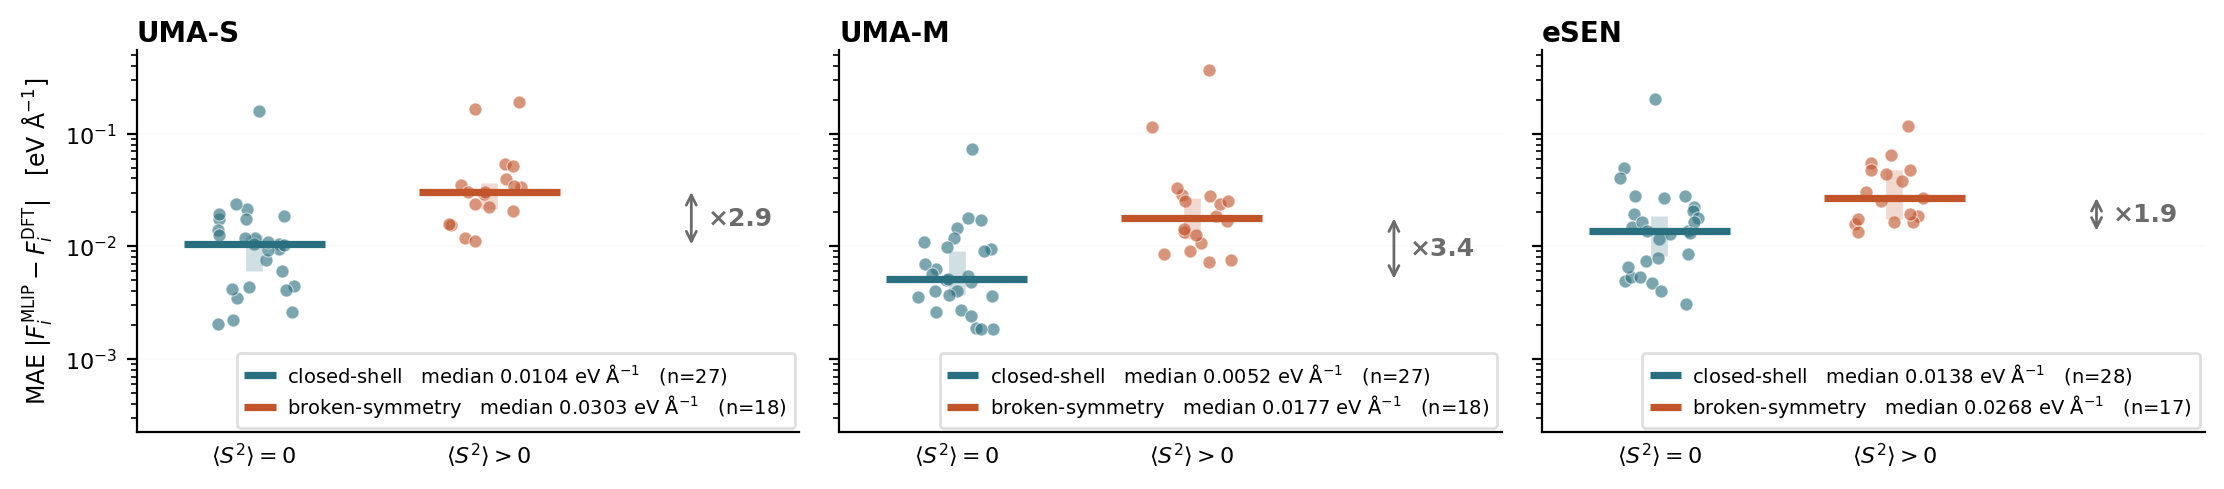
\includegraphics[width=\linewidth]{Pictures/fig2_force_mae.png}
  \caption{Force error at the transition state each model delivered:
  the absolute difference between model force and DFT force, averaged
  over all $3N$ Cartesian components, at the same unrelaxed geometry.
  DFT at the OMol25 level on the unrestricted surface
  (Sec.~\ref{sec:dft}); groups as in Fig.~\ref{fig:silent}. Dots are
  single structures, bars the group medians with their 95\,\% bootstrap
  intervals, and the arrow gives the ratio of the two medians.}
  \label{fig:ferr}
\end{figure}

The force error is larger at the broken-symmetry structures for every
model. Medians over the structures of each group, closed-shell against
broken-symmetry: 0.0104 against 0.0303~eV\,\AA$^{-1}$ for UMA-S,
0.0052 against 0.0177 for UMA-M and 0.0138 against 0.0268 for eSEN,
factors of 2.9, 3.4 and 1.9. Pooled over the three models the median
rises from 0.0095 to 0.0250~eV\,\AA$^{-1}$. This is a property of the model, not of the
search: the force error is measured at a fixed geometry, with no
optimisation involved.

The error does not depend on how deep the symmetry breaking is. The
breaking depth spans 0.6 to 3986~meV within the broken-symmetry group,
and the force error does not follow it (Spearman $\rho = -0.05$ over
the 53 structures). What matters is that a broken-symmetry solution
exists, not how far it lies below the restricted one.

In absolute terms the error stays small, and the two distributions overlap:
4 of the 53 broken-symmetry structures lie below the closed-shell median, 8 of
the 82 closed-shell structures above the broken-symmetry one. Small as it is,
the error sits at the transition state, and wrong forces there mean the model
cannot place it accurately. Section~\ref{sec:results-barrier} shows that this
has a meaningful effect on the barrier.


\subsection{The energy error is small and the geometry error is not}
\label{sec:results-barrier}

A model barrier can be wrong for two reasons. The model can assign the wrong
energy to a given structure, or it can place the transition state at the
wrong structure. Figure~\ref{fig:barrier} separates the two
(Table~\ref{tab:panels}).

\begin{figure}[!htbp]
  \centering
  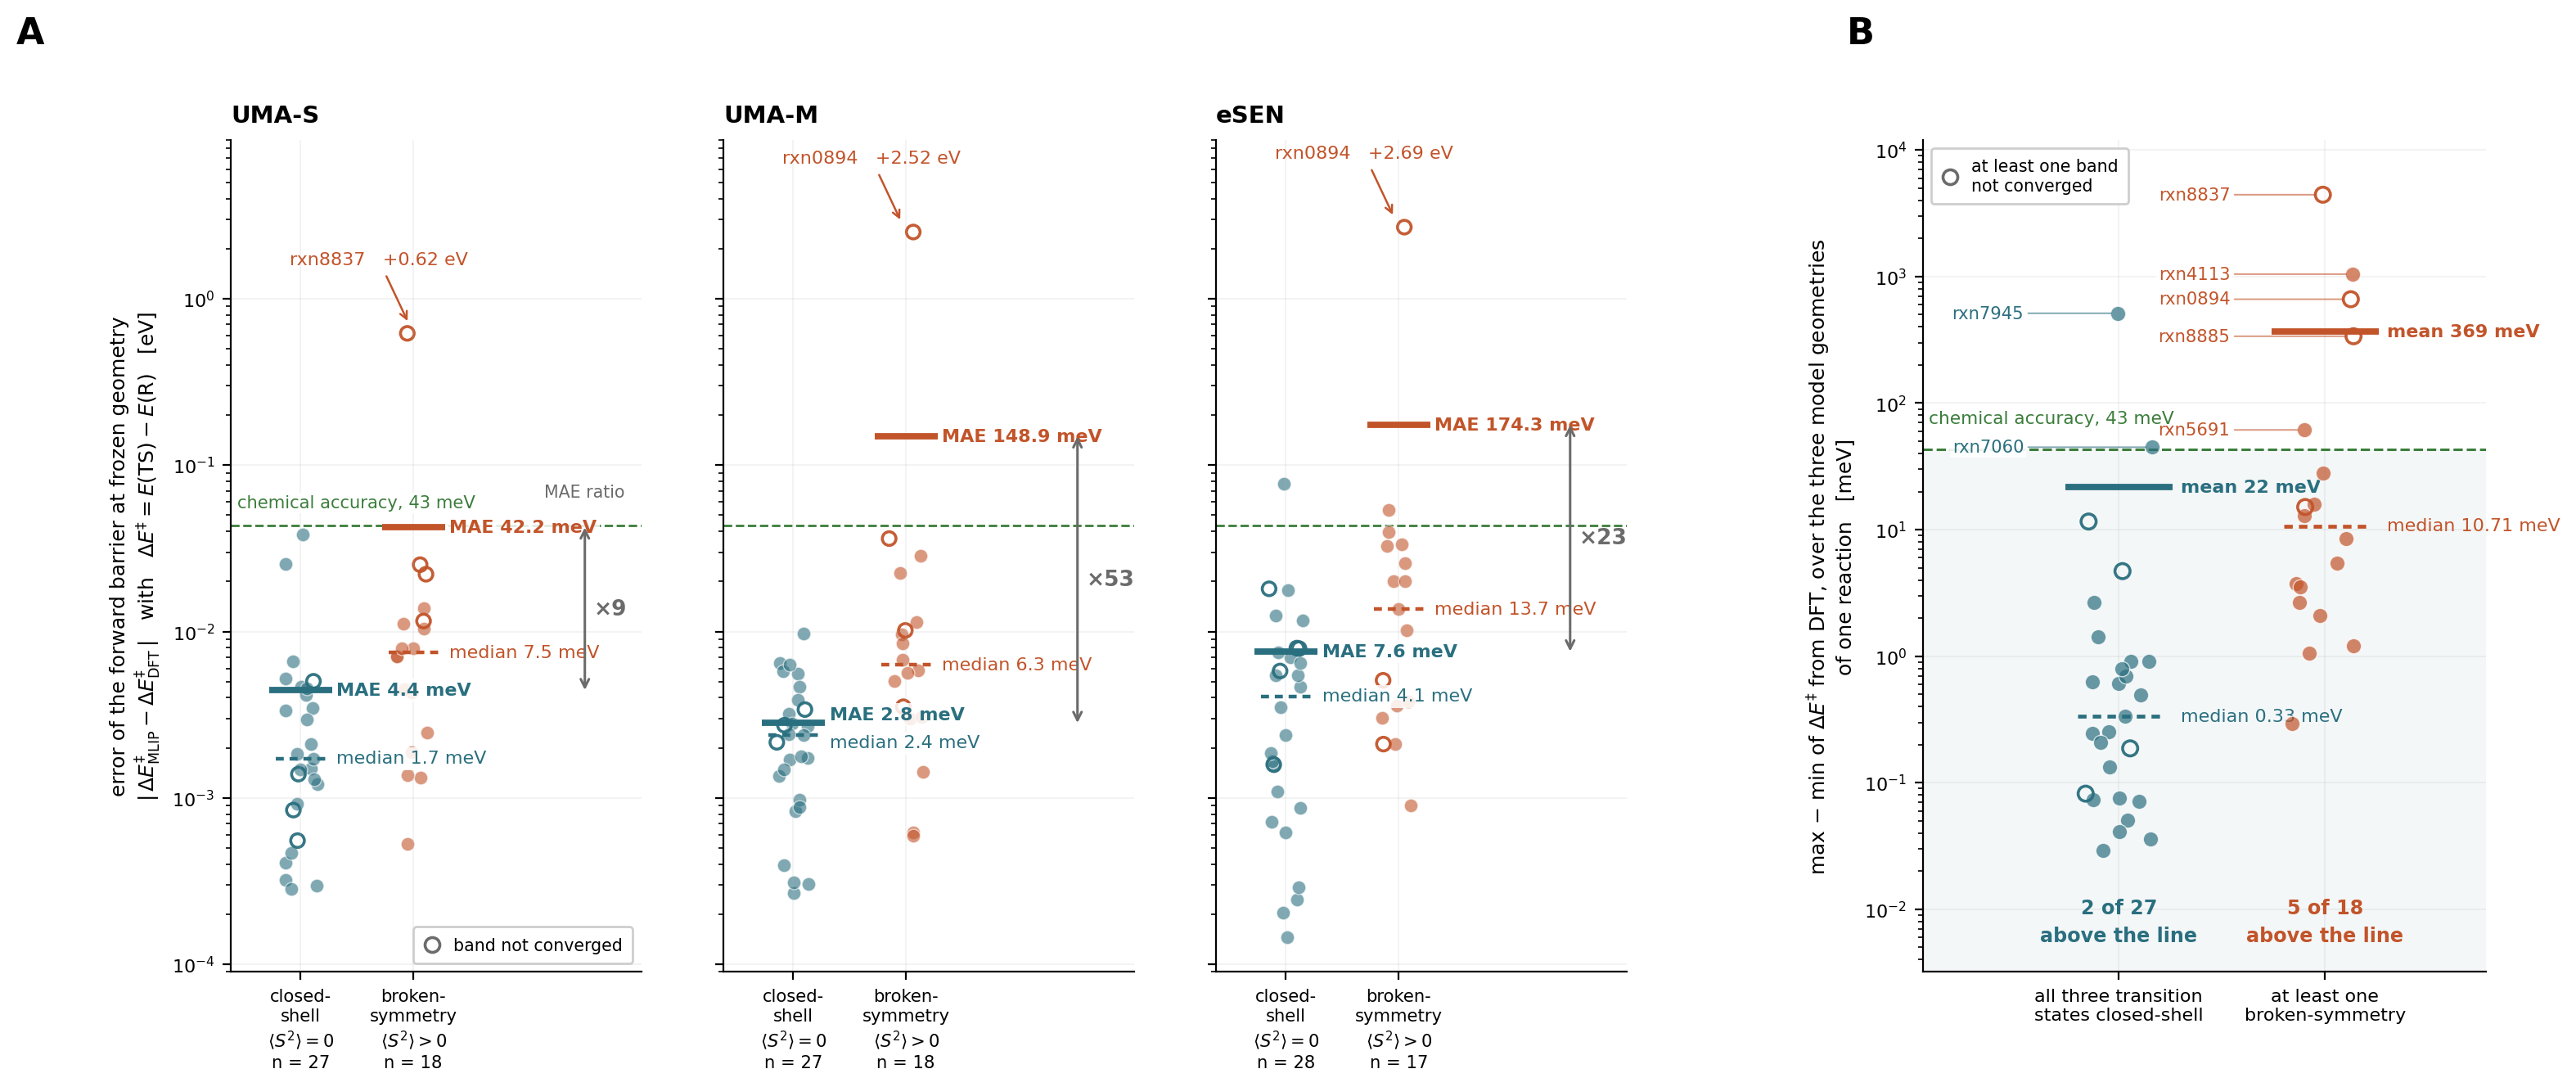
\includegraphics[width=\linewidth]{Pictures/fig3_v2.png}
  \caption{Energy error (A) and geometry error (B) of the model
  barriers. (A)~One dot per reaction and model: the barrier over that
  model's own structures, computed with the model and with DFT, and the
  absolute difference between the two. Solid bars are means, dashed bars
  medians; the named reaction sets the mean of each broken-symmetry group
  almost alone. (B)~One dot per reaction: the three DFT barriers over
  the structures of the three models, largest minus smallest. A reaction
  counts as broken-symmetry if at least one of its three transition
  states has $\langle S^2\rangle > 0$. The green line marks 1~kcal/mol
  (43~meV) for orientation. Open circles: the band of that search (A),
  or of at least one of the three searches of that reaction (B), did not
  reach the convergence criterion (Sec.~\ref{sec:neb}); all statistics
  include them. DFT at the OMol25 level on the unrestricted
  surface (Sec.~\ref{sec:dft}).}
  \label{fig:barrier}
\end{figure}

Panel~A isolates the energy error. It takes the reactant and the
transition state that one model found for a reaction and keeps both
geometries fixed. The barrier between them is computed twice, once with the model and once with DFT single
points. Since the geometries are the same in both, the two barriers
can differ only because the model's energies differ from DFT's. The
difference between them is the energy error.

Panel~B isolates the geometry error. The energy evaluation is fixed: DFT
for everything. The geometries vary: for each reaction, the three models
found three reactant and transition state pairs, and each pair gives a DFT
barrier. Since the energy method is the same for all three, the
barriers can differ only because the models stopped at different
geometries. The spread between them is the geometry error.

\begin{table}[H]
  \centering
  \small
  \caption{How the two panels of Fig.~\ref{fig:barrier} separate the two
  sources of barrier error. R = reactant, TS = transition state.}
  \label{tab:panels}
  \begin{tabular}{@{}lll@{}}
    \toprule
                          & Panel A                        & Panel B \\
    \midrule
    Structures (R, TS)    & from one model                 & from the three models \\
    Energy evaluated with & model \emph{and} DFT           & DFT only \\
    Barriers per reaction & 2 per model (6 in total)       & 3 \\
    Fixed                 & the structures                 & the energy function \\
    Varied                & the energy function            & the structures \\
    Plotted               & $|\Delta E^\ddagger_\mathrm{model} - \Delta E^\ddagger_\mathrm{DFT}|$
                          & $\max - \min$ of the three DFT barriers \\
    Measures              & energy error                   & geometry error \\
    \bottomrule
  \end{tabular}
\end{table}

Panel~A shows that the energy prediction of the model is not the
problem. The median error is 1.7,
2.4 and 4.1~meV on the closed-shell and 7.5, 6.3 and 13.7~meV on the
broken-symmetry structures, for UMA-S, UMA-M and eSEN, all well inside
chemical accuracy; 49 of the 53 broken-symmetry structures lie below 43~meV.
The mean absolute errors are 9, 53 and 23 times larger on the broken-symmetry
side, but one reaction per model sets them almost alone: rxn8837 misses by
$+0.62$~eV for UMA-S, rxn0894 by $+2.52$~eV for UMA-M and by $+2.69$~eV for
eSEN, all three from bands that did not converge. Apart from these three
cases and rxn8827 for eSEN, at 54~meV, the energies are right.

Panel~B shows that the different geometries do cause substantially
diverging barriers. The median spread is 0.33~meV at the closed-shell
reactions and 10.71~meV at the broken-symmetry ones, a factor of 32; the
means are 22 and 369~meV. Five of the 18 broken-symmetry reactions exceed
chemical accuracy, from 61~meV up to 4434~meV, against two of the 27
closed-shell ones, rxn7945 and rxn7060. So the large spreads sit
mostly, but not only, in the broken-symmetry group. The two reactions with the
largest energy error in Panel~A, rxn8837 and rxn0894, are also among the
three largest spreads in Panel~B. Three of the five, rxn8837, rxn0894
and rxn8885, are reactions whose bands did not converge. We therefore
repeat the comparison without the eight reactions in which at least one
of the three searches did not converge. In the remaining 37, the median
spread is 0.33~meV at the closed-shell reactions and 4.59~meV at the
broken-symmetry ones, a factor of 14. There, the spread exceeds 1~meV in
13 of the 14 broken-symmetry reactions but in only four of the 23
closed-shell ones, and it exceeds chemical accuracy in two reactions of
each group. The difference between the groups therefore does not come
from the unconverged searches, although they make it larger.

Together, the two panels say where the barrier error comes from. The energy
error is a few meV; the geometry error reaches electronvolts. The
models get the barrier wrong not because they misjudge the energy of
the structure they deliver, but because they deliver the wrong
structure. This has a practical consequence. A common
remedy for an inaccurate model energy is a DFT single point at the model
transition state. Here it corrects the energy, which was already right, and
keeps the geometry, which is wrong. The affected transition states have to
be re-optimised, and Fig.~\ref{fig:silent} has shown that the model's own
residual force does not tell which ones they are. The stability
analysis does: one unrestricted single point at the model transition
state identifies the broken-symmetry cases.

\subsection{The training geometries are furthest from stationarity where the models do worst}

The results so far concern the transition states the models deliver.
We now turn to the training geometries, to test whether the problems
the models have at broken-symmetry transition states can be traced back
to the training data. As described in Section~\ref{sec:labels}, we want
to know how far the stored transition states are from stationarity on
the label surface, the unrestricted surface at the OMol25 level. The
measure for this is the residual force. We measure it in three steps,
reported in Table~\ref{tab:ladder}, and each step tells one thing.

\begin{table}[H]
  \centering
  \small
  \setlength{\tabcolsep}{5pt}
  \caption{Median residual force at the 45 stored Transition1x
  transition states, one change per step: the level in step 2, the
  spin formalism in step 3 (Section~\ref{sec:labels}); numbers in
  parentheses are reaction counts. $^{a}$Lowest unrestricted solution
  (Sec.~\ref{sec:dft}). For the closed-shell group it coincides with
  the restricted one, so the last two columns are equal there.}
  \label{tab:ladder}
  \begin{tabular}{@{}lccc@{}}
    \toprule
    & \multicolumn{3}{c}{median residual force [eV\,\AA$^{-1}$]} \\
    \cmidrule(l){2-4}
    & step 1 & step 2 & step 3 \\
    & $\omega$B97X/6-31G(d) & $\omega$B97M-V/def2-TZVPD & $\omega$B97M-V/def2-TZVPD \\
    & restricted & restricted & unrestricted$^{a}$ \\
    & as relaxed & level changed & spin formalism changed \\
    \midrule
    \multicolumn{4}{@{}l}{\emph{Transition1x transition states, relaxed at the Transition1x level} (45)} \\
    \quad closed-shell (27)     & $0.0147$ & $0.609$ & $0.609$ \\
    \quad broken-symmetry (18)  & $0.0138$ & $0.589$ & $1.636$ \\
    \bottomrule
  \end{tabular}
\end{table}

Step 1 shows that the stored geometries are transition states at
their own level, so nothing was off before relabelling. Step 2 shows
that changing the level takes both groups equally far from
stationarity, so the level cannot be what separates the groups. Step 3
shows that changing the spin formalism affects only the broken-symmetry
group, and by a lot: that is the separation. The closed-shell group
shows what the level change alone does: its training points are equally
far from stationarity, and the models still find its transition states.
The broken-symmetry group has the spin-formalism change on top, its
training points carry almost three times the residual force, and there
the models do worse.

\paragraph{Control.} \emph{Re-optimised restricted at the OMol25 level, the
geometries are transition states of the restricted surface ($0.039$
and $0.042$), and on the unrestricted surface the broken-symmetry group
is still far from stationarity, $1.87$, a factor of $32$: the transition state of a path
relaxed restricted is not a transition state of the unrestricted
surface, at whichever level it is relaxed.}


\subsection{Discussion}
\label{sec:omol-discussion}

\paragraph{Summary of the results.} The models perform well at locating
closed-shell transition states and worse across all metrics at locating
broken-symmetry ones.

\paragraph{Answer to RQ2.} The models locate the closed-shell
transition states although their training paths were relaxed at another
level: when only the level of theory changes, relabelling the paths
without re-optimising them is sufficient. At broken-symmetry
transition states, where the spin formalism changes as well, the models
still reproduce the energies but deliver structures that are not
stationary points of the unrestricted surface, with force errors two to
three times larger. The answer to RQ2 is therefore yes for a change of
level, and not reliably once the spin formalism changes with it.

\paragraph{Robustness of the finding.} The difference between the two
groups is not a convergence artefact: the force error is measured at
fixed geometries, with no optimisation involved. Nor do the models
misjudge the energies: at the structures they deliver, the energies are
within chemical accuracy for almost all of them, so the problem lies in
the forces and the geometry.

\paragraph{Multireference character and broken symmetry.} The
broken-symmetry reactions are also the reactions of highest
multireference character, so the difference between the groups could be
an effect of multireference character alone. Part of it is. Among the
closed-shell structures, where no broken symmetry is involved, the
median DFT residual force at the model transition state rises from
0.030~eV\,\AA$^{-1}$ in the low-MR tier to 0.082 in the high-MR tier,
and the force error from 0.004 to 0.018.\footnote{In the high-MR tier,
28 of the 78 model transition states are closed-shell and 50
broken-symmetry; the low-MR tier holds 30, all closed-shell.}
Chapter~\ref{ch:delta} saw the same dependence in MACE on its own level.
Broken symmetry adds to this. Within the $N_\mathrm{FOD}$ range that
both groups share (0.70 to 0.90, medians 0.79 and 0.78; 28 closed-shell
and 29 broken-symmetry structures), the broken-symmetry structures
remain worse, 0.137 against 0.082 in residual force and 0.028 against
0.018 in force error, a factor of about 1.6. The two effects also behave
differently. Within the closed-shell group the error rises with
$N_\mathrm{FOD}$ (Spearman $\rho = 0.61$ for the residual force and
$0.73$ for the force error over all 82 structures); within the
broken-symmetry group it does not ($\rho = -0.17$ and $-0.22$ over all
53). Multireference character acts continuously, whereas broken
symmetry acts as a step that comes with the existence of the lower
solution. The pooled factor of 2.5 between the two groups therefore
contains both effects, and the factor of about 1.6 is the part that
belongs to broken symmetry itself. It rests on ten reactions on either
side.

\paragraph{Explanation, and what remains open.} The training data offer
an explanation. On the label surface the stored transition states of
the broken-symmetry reactions carry a median residual force of
$1.64$~eV\,\AA$^{-1}$, against $0.61$ for the closed-shell ones, and it
is the change of spin formalism, not the change of level, that
separates the groups (Table~\ref{tab:ladder}).\footnote{The same holds
at equal multireference character: in the $N_\mathrm{FOD}$ range that
both groups share, the stored transition states of the broken-symmetry
reactions carry 1.70~eV\,\AA$^{-1}$, against 0.58 for the closed-shell
ones.} The difference is one of
degree: the closed-shell training points are not stationary on the
label surface either, and the models still find those transition
states. That the larger distance from stationarity causes the larger
errors is one likely explanation; it has not been tested by training on
paths relaxed unrestricted. The training data are also not the only
candidate. Where the broken-symmetry solution sets in, the curvature of
the unrestricted surface changes abruptly, and a smooth model may fit
that region poorly whatever the training geometries are. Each candidate makes a prediction inside the broken-symmetry group. If
the training data are the cause, the reactions whose training points
are furthest from stationarity should show the largest errors. They do
not (Spearman $\rho = -0.30$ over the 18 reactions). If the shape of the
surface is the cause, the error should be largest close to the onset of
symmetry breaking and fade with growing breaking depth. It does so only
in part: the force error stays level up to a breaking depth of about
1.3~eV and falls to the closed-shell level above it. With 18 reactions
neither observation is conclusive, and between the two groups the
training data fit. Both causes may contribute.

\paragraph{Other reactive data in OMol25.} Transition1x is not the only
reactive data in OMol25, and one might object that the models learned
the broken-symmetry saddles elsewhere. They could not. No reaction
path in OMol25 was relaxed at the level the labels use~\cite{omol25}.
The Transition1x bands were relaxed at \mbox{$\omega$B97X/6-31G(d)}.
The RGD1 transition states were optimised at B3LYP-D3/TZVP for
closed-shell species~\cite{zhao2023rgd1}, and OMol25 interpolated
between reactant, transition state and product rather than relaxing a
path. The reaction paths OMol25 generated itself come from
artificial-force searches on a machine-learned potential and from path
interpolation, started from force-field geometries, and were not
relaxed on a DFT surface. ANI-1xBB~\cite{zhang2025ani1xbb} was labelled
unrestricted as well, but it consists of constrained bond-stretching
scans and molecular-dynamics snapshots and contains no transition-state
search. The models have therefore seen broken-symmetry labels along
dissociating bonds, but a saddle of the unrestricted surface at the
OMol25 level does not exist in the training data.

\paragraph{Composition of the benchmark.} The sample is 45 CHNO reactions
selected for multireference character, three models and 135 searches.
The high-MR tier is where broken-symmetry transition states were
expected and found. The findings concern this class of reactions, not
OMol25 as a whole. The 135 structures are three searches each of 45
reactions, 18 of them broken-symmetry, so they are not 135 independent
observations.

\paragraph{Practical implications.} A DFT single point at the model transition state
does not repair it: it corrects the energy, which was right, and keeps
the geometry, which is wrong. The affected transition states have to
be re-optimised on the unrestricted surface, and the stability
analysis identifies them.

\paragraph{Implications for the models.} Re-optimising repairs a single
search, not the models. What would repair the models depends on the
cause of their errors. If the training data
are the cause, training paths re-optimised on the unrestricted surface
should remove the errors; if the shape of the unrestricted surface is
the cause, they should not. This has not been tested.
Chapter~\ref{ch:conclusion} takes this up.
